\documentclass[12pt]{article}
\usepackage{amsmath} % AMS Math Package
\usepackage{bm}
\usepackage{amsthm} % Theorem Formatting
\usepackage{amssymb}    % Math symbols such as \mathbb
\usepackage{graphicx} % Allows for eps images
\usepackage[dvips,letterpaper,margin=1in,bottom=0.7in]{geometry}
\usepackage{tensor}
\usepackage{amsmath}
\usepackage{siunitx}
\usepackage{physics}
\usepackage{amsmath, amssymb, graphics, setspace}

\newcommand{\mathsym}[1]{{}}
\newcommand{\unicode}[1]{{}}

\newcounter{mathematicapage}

\newtheorem{p}{Problem}
\usepackage{cancel}
\newtheorem*{lem}{Lemma}
\theoremstyle{definition}
\newtheorem*{dfn}{Definition}
 \newenvironment{s}{%\small%
        \begin{trivlist} \item \textbf{Solution}. }{%
            \hspace*{\fill} $\blacksquare$\end{trivlist}}%


\begin{document}

 {\noindent\Huge\bf  \\[0.5\baselineskip] {\fontfamily{cmr}\selectfont  Homework 3}         }\\[2\baselineskip] % Title
{ {\bf \fontfamily{cmr}\selectfont Quantum Mechanics}\\ {\textit{\fontfamily{cmr}\selectfont     Sept 15th, 2022}}}~~~~~~~~~~~~~~~~~~~~~~~~~~~~~~~~~~~~~~~~~~~~~~~~~~~~~~~~~~~~~~~~~~~~~~~~~~~~~    {\large \textsc{Clayton Seitz}
\\[1.4\baselineskip] 

\begin{p}
Problem 2.1 from Sakurai
\end{p}

\begin{s}
The Heisenberg equation of motion reads

\begin{align*}
\frac{dA}{dt} = \frac{1}{i\hbar}\left[A,H\right]
\end{align*}

For the spin precession problem, we have the Hamiltonian

\begin{align*}
H = -\left(\frac{eB}{mc}\right)S_{z} = \omega S_{z}
\end{align*}

For $A = S_{x},S_{y},S_{z}$, the time evolution is given by

\begin{align*}
\frac{dS_{x}}{dt} &= \frac{\omega}{i\hbar}\left[S_{x},S_{z}\right] = -\omega S_{y}\\
\frac{dS_{y}}{dt} &= \frac{\omega}{i\hbar}\left[S_{y},S_{z}\right] = \omega S_{x}\\
\frac{dS_{z}}{dt} &= \frac{\omega}{i\hbar}\left[S_{z},S_{z}\right] = 0
\end{align*}

The above system has a straightforward solution:

\begin{align*}
S_{x}(t) &= \cos(\omega t)\\
S_{y}(t) &= \sin(\omega t)\\
S_{z}(t) &= S_{z}(0)
\end{align*}


\end{s}

\begin{p}
Problem 2.3 from Sakurai
\end{p}

\begin{s}
We are given that $\vec{B} = B\hat{z}$ and that we are in the eigenstate $\ket{\psi(0)} = \ket{\bm{S}\cdot \bm{\hat{n}}}_{+}$, which reads

\begin{align*}
\ket{\psi(0)} &= \psi_{+}\ket{+} + \psi_{-}\ket{-}\\
&= \cos{\frac{\beta}{2}}\ket{+} + \sin{\frac{\beta}{2}}\ket{-}\\
\end{align*}

where we have set $\alpha=0$ since the ket is in the x-z plane. This state will evolve according to a Hamiltonian

\begin{align*}
H = -\left(\frac{eB}{m_{e}c}\right)S_{z}
\end{align*}

Let $\omega = |e|B/m_{e}c$ giving $H=\omega S_{z}$. We have the energies

\begin{align*}
E_{\pm} = \mp \frac{e\hbar B}{2m_{e}c} = \mp \hbar\omega
\end{align*}

\begin{align*}
\ket{\psi(t)} &= \psi_{+}(0)\exp\left(\frac{-iE_{+}t}{\hbar}\right)\ket{+} + \psi_{-}(0)\exp\left(\frac{-iE_{-}t}{\hbar}\right)\ket{-}\\
&= \cos{\frac{\beta}{2}}\exp\left(\frac{-i\omega t}{2}\right)\ket{+} + \sin{\frac{\beta}{2}}\exp\left(\frac{i\omega t}{2}\right)\ket{-}
\end{align*}

In general, the probability of measuring $\ket{+}_{x} = \frac{1}{\sqrt{2}}\ket{+} + \frac{1}{\sqrt{2}}\ket{-}$ is given by the inner product

\begin{align*}
|\bra{S_{x};+}\ket{\psi;t}|^{2} &= \bigg|\left(\frac{1}{\sqrt{2}}\bra{+} + \frac{1}{\sqrt{2}}\bra{-}\right)\cdot\\
&\left(\psi_{+}\exp\left(\frac{-i\omega t}{2}\right)\ket{+} + \psi_{-}\exp\left(\frac{i\omega t}{2}\right)\ket{-}\right)\bigg|^{2}\\
&= \bigg|\frac{1}{\sqrt{2}}\cos\frac{\beta}{2}\exp\left(\frac{-i\omega t}{2}\right)+\frac{1}{\sqrt{2}}\sin\frac{\beta}{2}\exp\left(\frac{i\omega t}{2}\right)\bigg|^{2}
\end{align*}

Using the half-angle identity for $\sin\theta$ and some straightforward arithmetic gives

\begin{align*}
|\bra{S_{x};+}\ket{\psi;t}|^{2} &= \frac{1+\sin\beta\cos\omega t}{2}
\end{align*}


For the time-dependence of $\langle S_{x}\rangle$, we have

\begin{align*}
\langle S_{x}\rangle(t) &= \bra{\psi;t}S_{x}\ket{\psi;t}\\
&= \left(\psi_{+}\exp\left(\frac{i\omega t}{2}\right)\bra{+} + \psi_{-}\exp\left(\frac{-i\omega t}{2}\right)\bra{-}\right)\\
&\cdot \frac{\hbar}{2} \left(\psi_{+}\exp\left(-\frac{i\omega t}{2}\right)\ket{-} + \psi_{-}\exp\left(\frac{i\omega t}{2}\right)\ket{+}\right)
\end{align*}

Subsituting $\psi_{+}$ and $\psi_{-}$ with the same values as above, we get

\begin{align*}
\langle S_{x}\rangle(t) &= \frac{\hbar}{2}\sin\beta\cos\omega t
\end{align*}

When $\beta = \pi /2$ the probability oscillates between 0 and 1 with frequency $\omega$ and when $\beta = 0$ then the probability is always $1/2$, as expected. The expectation value also makes sense because when $\beta = 0$, we can get $\pm \hbar /2$ with equal probability, giving zero on average. When $\beta = \pi /2$ the expectation value oscillates between $\hbar /2$ and $-\hbar /2$.

\end{s}

\begin{p}
Problem 2.9 from Sakurai
\end{p}

\begin{s}

We were given the wavefunction 

\begin{align*}
\bra{x}\ket{\alpha} = A(x-a)^{2}(x+a)^{2}\exp(ikx)
\end{align*}

We can start by visualizing the real and imaginary parts of the position representation $\bra{x}\ket{\alpha}$ when $A=a=k=1$


\begin{doublespace}
\noindent\(\pmb{\text{Plot}\left[(x-1)^2 (x+1)^2 \text{Cos}[x],\{x,-2,2\}\right]}\)
\end{doublespace}

\includegraphics{test_gr1.eps}

\begin{doublespace}
\noindent\(\pmb{\text{Plot}\left[(x-1)^2 (x+1)^2 \text{Sin}[x],\{x,-2,2\}\right]}\)
\end{doublespace}

\includegraphics{test_gr2.eps}

To find the normalization constant $A$, we just need to integrate $\bra{x}\ket{\alpha}$

\begin{align*}
A &= \left(\int_{-a}^{+a}\bra{x}\ket{\alpha}dx\right)^{-1}\\
&= \left(\int_{-a}^{+a}(x-a)^{2}(x+a)^{2}\exp(ikx)dx\right)^{-1}\\
&= \left(\int_{-a}^{+a}(x-a)^{2}(x+a)^{2}\cos(kx)dx\right)^{-1}\\
&- \left(\int_{-a}^{+a}(x-a)^{2}(x+a)^{2}\sin(kx)dx\right)^{-1}
\end{align*}

We can evalulate these integrals individually:

\begin{doublespace}
\noindent\(\pmb{\text{Integrate}\left[(x-a)^2 (x+a)^2 \text{Cos}[k*x],\{x,-a,a\}\right]}\)
\end{doublespace}

\begin{doublespace}
\noindent\(-\frac{16 \left(3 a k \text{Cos}[a k]+\left(-3+a^2 k^2\right) \text{Sin}[a k]\right)}{k^5}\)
\end{doublespace}

\begin{doublespace}
\noindent\(\pmb{\text{Integrate}\left[(x-a)^2 (x+a)^2 \text{Sin}[k*x],\{x,-a,a\}\right]}\)
\end{doublespace}

\begin{doublespace}
\noindent\(0\)
\end{doublespace}

The integral of the imaginary part is obvious since that part of the wavefunction is odd.

\begin{align*}
A = -\frac{k^5}{16 \left(3ka\cos(ka)+\left(a^2 k^2-3\right) \sin(ka)\right)}
\end{align*}

The expectation value $\langle x\rangle$ is found by integrating

\begin{align*}
\langle x \rangle &= \int_{-a}^{a} x\bra{\alpha}\ket{x}\bra{x}\ket{\alpha}dx \\
&= \int_{-a}^{+a} x\bra{\alpha}\ket{x}\bra{x}\ket{\alpha}dx \\
&= \int_{-a}^{+a} x (x-a)^{2}(x+a)^{2}dx
\end{align*}

where the complex exponential vanishes due to the complex conjugation. The expectation value $\langle x^{2}\rangle$ is found by integrating

\begin{align*}
\langle x^{2} \rangle &= \int_{-a}^{+a} x^{2} (x-a)^{2}(x+a)^{2}dx
\end{align*}

The expectation value $\langle p\rangle$ is found similarly

\begin{align*}
\langle p \rangle &= \int_{-a}^{+a} \bra{\alpha}\ket{x}\frac{\hbar}{i}\frac{\partial}{\partial x}\bra{x}\ket{\alpha}dx\\
&= A^{2} \int_{-a}^{+a}(x-a)^{2}(x+a)^{2}\exp(-ikx)\frac{\hbar}{i}\frac{\partial}{\partial x}(x-a)^{2}(x+a)^{2}\exp(ikx)
\end{align*}

The expectation value $\langle p^{2}\rangle$ is found by integrating

\begin{align*}
\langle p^{2} \rangle &= -\int_{-a}^{+a} \bra{\alpha}\ket{x}\hbar^{2}\frac{\partial^{2}}{\partial x^{2}}\bra{x}\ket{\alpha}dx\\
&= -A^{2}\int_{-a}^{+a}(x-a)^{2}(x+a)^{2}\exp(-ikx)\hbar^{2}\frac{\partial^{2}}{\partial x^{2}}(x-a)^{2}(x+a)^{2}\exp(ikx)
\end{align*}

The variance $\langle (\Delta x)^{2}\rangle$ is just


\begin{align*}
\langle (\Delta x)^{2}\rangle = \langle x^{2} \rangle - \langle x \rangle^{2}
\end{align*}

The variance $\langle (\Delta p)^{2}\rangle$ is just


\begin{align*}
\langle (\Delta p)^{2}\rangle = \langle p^{2} \rangle - \langle p \rangle^{2}
\end{align*}


\end{s}

\begin{p}
Problem 2.10 from Sakurai
\end{p}

\begin{s}
Let $\ket{\psi}=\alpha\ket{a'} + \beta\ket{a''}$ be an eigenvector of the Hamiltonian. Note that this must be real for the eigenvalue to be real. That means that

\begin{align*}
H\ket{\psi} &= \left(\ket{a'}\delta\bra{a''} + \ket{a''}\delta\bra{a'}\right)\left(\alpha\ket{a'} + \beta\ket{a''}\right)\\
&= \delta\left(\alpha\ket{a''} + \beta\ket{a'}\right)
\end{align*}

Therefore $\alpha = \beta = \frac{1}{\sqrt{2}}$ or $\alpha=\frac{1}{\sqrt{2}}$ and $\beta=-\frac{1}{\sqrt{2}}$. Giving eigenvalues $\pm \delta$. To get the time evolution of the state, we need to express these in the basis of $H$. Just based on inspection of the the two bases, we can tell that

\begin{align*}
\ket{a'} &= \frac{1}{\sqrt{2}}\left(\ket{\psi_{1}}-\ket{\psi_{2}}\right)\\
\ket{a''} &= \frac{1}{\sqrt{2}}\left(\ket{\psi_{1}}+\ket{\psi_{2}}\right)
\end{align*}

and, since the Hamiltonian is time-independent, a state prepared in $\ket{a'}$ will evolve according to 

\begin{align*}
\ket{\alpha(t)} = \frac{1}{\sqrt{2}}\exp\left(\frac{-i\delta t}{\hbar}\right)\ket{\psi_{1}} - \frac{1}{\sqrt{2}}\exp\left(\frac{i\delta t}{\hbar}\right)\ket{\psi_{2}}
\end{align*}

The probability of finding the system in the state $\ket{a''}$ at a later time is

\begin{align*}
|\bra{a''}\ket{\alpha(t)}|^{2} &= \bigg|\frac{1}{\sqrt{2}}\left(\bra{\psi_{1}}+\bra{\psi_{2}}\right)\\
&\cdot \left(\frac{1}{\sqrt{2}}\exp\left(\frac{-i\delta t}{\hbar}\right)\ket{\psi_{1}} - \frac{1}{\sqrt{2}}\exp\left(\frac{i\delta t}{\hbar}\right)\ket{\psi_{2}}\right)\bigg|^2\\
&= \frac{1}{4}\sin^{2}\frac{\delta t}{\hbar}
\end{align*}

This could describe a system in which the eigenvectors of the Hamiltonian are simultaneous with the eigenvectors of $S_{x}$, however the states $\ket{a'}$ and $\ket{a''}$ are expressed in the $S_{z}$ basis.

\end{s}

\begin{p}
Problem 2.12 from Sakurai
\end{p}

\begin{s}
The state is prepared in 

\begin{align*}
\ket{\alpha;t=0} = \frac{1}{\sqrt{2}}\ket{0} + \frac{\exp(i\delta)}{\sqrt{2}}\ket{1}
\end{align*}

In general, the energies of $\ket{n}$ are $E_{n} = \left(n+\frac{1}{2}\right)\hbar\omega$. Therefore, the time dependence of the state can be evalulated as

\begin{align*}
\ket{\alpha;t} &= \exp\left(-\frac{iHt}{\hbar}\right)\ket{\alpha;t}\\
&= \frac{1}{\sqrt{2}}\exp\frac{-i\omega t}{2}\ket{0} + \frac{1}{\sqrt{2}}\exp(i\delta)\exp\frac{-3i\omega t}{2}\ket{1}
\end{align*}

\begin{align*}
\bra{x}\ket{\alpha;t} = \frac{1}{\sqrt{2}}\exp\frac{-i\omega t}{2}\bra{x}\ket{0} + \frac{1}{\sqrt{2}}\exp(i\delta)\exp\frac{-3i\omega t}{2}\bra{x}\ket{1}
\end{align*}

and we know in general that the position representation of $\ket{n}$ i.e., $\bra{x}\ket{n}$ are

\begin{align*}
\bra{x}\ket{n} = \psi _{n}(x)={\frac {1}{\sqrt {2^{n}\,n!}}}\left({\frac {m\omega }{\pi \hbar }}\right)^{1/4}e^{-{\frac {m\omega x^{2}}{2\hbar }}}H_{n}\left({\sqrt {\frac {m\omega }{\hbar }}}x\right)
\end{align*}


\begin{align*}
\langle x\rangle(t) &= \bra{\alpha;t}x\ket{\alpha;t}\\
&= \left(\frac{1}{\sqrt{2}}\exp\frac{i\omega t}{2}\bra{0} + \frac{1}{\sqrt{2}}\exp(-i\delta)\exp\frac{3i\omega t}{2}\bra{1}\right) \\
&x \left(\frac{1}{\sqrt{2}}\exp\frac{-i\omega t}{2}\ket{0} + \frac{1}{\sqrt{2}}\exp(i\delta)\exp\frac{-3i\omega t}{2}\ket{1}\right)\\
&= \frac{1}{2}\bra{0}x\ket{0} + \frac{1}{2}\bra{1}x\ket{1} \\
&+ \frac{1}{2}\exp(i\delta)\exp(-i\omega t)\bra{0}x\ket{1} + \frac{1}{2}\exp(-i\delta)\exp(i\omega t)\bra{1}x\ket{0}
\end{align*}

Now recall the general expression for the matrix element of $x$

\begin{align*}
\bra{n'}x\ket{n} = \sqrt{\frac{\hbar}{2m\omega}}\left(\sqrt{n}\delta_{n',n-1} +\sqrt{n+1}\delta_{n',n+1}\right)
\end{align*}

which means that the above expression simplifies to 

\begin{align*}
\langle x\rangle(t) &= \frac{1}{2}\exp(i\delta)\exp(-i\omega t)\bra{0}x\ket{1} + \frac{1}{2}\exp(-i\delta)\exp(i\omega t)\bra{1}x\ket{0}\\
&= \frac{1}{2}\sqrt{\frac{\hbar}{2m\omega}}\left(\exp(i\delta)\exp(-i\omega t)+\exp(-i\delta)\exp(i\omega t)\right)\\
&= \sqrt{\frac{\hbar}{2m\omega}}\cos(\delta-\omega t)\\
&= \sqrt{\frac{\hbar}{2m\omega}}\cos(\omega t-\delta)
\end{align*}

For momentum, we can just replace the operator $x$ with $p$ in the expressions above:

\begin{align*}
\langle p\rangle(t) &= \bra{\alpha;t}x\ket{\alpha;t}\\
&= \left(\frac{1}{\sqrt{2}}\exp\frac{i\omega t}{2}\bra{0} + \frac{1}{\sqrt{2}}\exp(-i\delta)\exp\frac{3i\omega t}{2}\bra{1}\right) \\
&\hat{p} \left(\frac{1}{\sqrt{2}}\exp\frac{-i\omega t}{2}\ket{0} + \frac{1}{\sqrt{2}}\exp(i\delta)\exp\frac{-3i\omega t}{2}\ket{1}\right)\\
&= \frac{1}{2}\bra{0}p\ket{0} + \frac{1}{2}\bra{1}p\ket{1} \\
&+ \frac{1}{2}\exp(i\delta)\exp(-i\omega t)\bra{0}p\ket{1} + \frac{1}{2}\exp(-i\delta)\exp(i\omega t)\bra{1}p\ket{0}
\end{align*}

and we have another general expression for the matrix element of $p$

\begin{align*}
\bra{n'}p\ket{n} = i\sqrt{\frac{m\hbar\omega}{2}}\left(-\sqrt{n}\delta_{n',n-1} +\sqrt{n+1}\delta_{n',n+1}\right)
\end{align*}

which again means that the above expression simplifies to 

\begin{align*}
\langle p\rangle(t) &= \frac{1}{2}\exp(i\delta)\exp(-i\omega t)\bra{0}p\ket{1} + \frac{1}{2}\exp(-i\delta)\exp(i\omega t)\bra{1}p\ket{0}\\
&= \frac{i}{2}\sqrt{\frac{m\hbar\omega}{2}}\left(-\exp(i\delta)\exp(-i\omega t)+\exp(-i\delta)\exp(i\omega t)\right)\\
&= -\sqrt{\frac{m\hbar\omega}{2}}\sin(\omega t - \delta)
\end{align*}

In the Heisenberg picture, we have the Heisenberg equations of motion

\begin{align*}
\frac{dp}{dt} &= -m\omega^{2}x\\
\frac{dx}{dt} &= \frac{p}{m}
\end{align*}

It is has been shown in the text how to uncouple these in terms of the ladder operators and solve the system for the time dependent operators $x(t)$ and $p(t)$

\begin{align*}
x(t) &= x(0)\cos(\omega t) + \left(\frac{p(0)}{m\omega}\right)\sin(\omega t)\\
p(t) &= -m\omega x(0)\sin(\omega t) + p(0)\cos(\omega t)
\end{align*}

To get $\langle x \rangle (t)$ we have

\begin{align*}
\langle x \rangle (t) &= \bra{\alpha} x(0)\cos(\omega t) + \left(\frac{p(0)}{m\omega}\right)\sin(\omega t) \ket{\alpha}\\
&= \bra{\alpha}x(0)\ket{\alpha}\cos(\omega t) + \bra{\alpha} p(0)\ket{\alpha}\frac{\sin(\omega t)}{m\omega}
\end{align*}

\begin{align*}
\bra{\alpha}x(0)\ket{\alpha} &= \frac{1}{2}\bra{0}x(0)\ket{0} + \frac{1}{2}\bra{1}x(0)\ket{1} \\
&+ \frac{1}{2}\exp(i\delta)\bra{0}x(0)\ket{1}+ \frac{1}{2}\exp(i\delta)\bra{1}x(0)\ket{0}\\
&= \sqrt{\frac{\hbar}{2m\omega}}\exp(i\delta)
\end{align*}

The factor of one-half disappeared in the $\bra{\alpha}x(0)\ket{\alpha}$ term since $\bra{n'}x\ket{n}$ is real and therefore equal to its complex conjugate


\begin{align*}
\langle x \rangle (t) &= \sqrt{\frac{\hbar}{2m\omega}}\exp(i\delta)\cos(\omega t) + \frac{i}{2}\exp(i\delta)\sqrt{\frac{m\hbar\omega}{2}}\frac{\sin(\omega t)}{m\omega}\\
&= \sqrt{\frac{\hbar}{2m\omega}}\exp(i\delta)\exp(i\omega t)\\
&= \sqrt{\frac{\hbar}{2m\omega}}\exp(i(\omega t+\delta))
\end{align*}


\end{s}

\begin{p}
Problem 2.13 from Sakurai
\end{p}

\begin{s}

The Heisenberg equations of motion are

\begin{align*}
\frac{dp}{dt} &= F\\
\frac{dx}{dt} &= \frac{p_{0}+Ft}{m}
\end{align*}

The solution is simply

\begin{align*}
p(t) &= p(0) + Ft\\
x(t) &= x(0) + \frac{p(0)}{m}t + \frac{1}{2}\frac{Ft^{2}}{m}
\end{align*}

\begin{align*}
\langle x \rangle (t) &= \bra{\alpha} \left(x(0) + \frac{p_{0}}{m}t + \frac{1}{2}\frac{Ft^{2}}{m}\right)\ket{\alpha}\\
&= x_{0} + \frac{p_{0}t}{m} + \frac{Ft^{2}}{2m}
\end{align*}

and for $\langle p\rangle$ we have

\begin{align*}
\langle p \rangle (t) &= \bra{\alpha} p(0) + Ft\ket{\alpha}\\
&= p_{0} + Ft
\end{align*}

In the Schrodinger picture, this Hamiltonian is not a constant

\begin{align*}
H(t) = \frac{p(t)^{2}}{2m} + V(x,t) = \frac{p(t)^{2}}{2m} + Fx(t)
\end{align*}

although, using the canonical commutation relations, we can see that $H(t_{0})$ commutes with $H(t)$. So we should be able to define

\begin{align*}
\mathcal{U}(t,t_{0}) = \exp\left(-\frac{i}{\hbar}\int_{t_{0}}^{t} H(t)dt\right)
\end{align*}

such that $\ket{\alpha;t} = \mathcal{U}(t,t_{0}) \ket{\alpha;t_{0}}$. If we evaluated that expression, then we could write $\ket{\alpha;t}$ explicitly.

\end{s}



\end{document}